\documentclass[11pt]{report}
\usepackage{graphicx}
\usepackage{hyperref}
\begin{document}
\begin{titlepage}
    \thispagestyle{empty}
    \title{%
    Toxic Processor \\
    \large A simplistic 4-bit processor ready to synthesis \\ 
    Version 2.0.0}
    \author{Entropy Xu \\ 
            \href{mailto:entropy.xcy@protonmail.com}{entropy.xcy@protonmail.com} }
    \maketitle
    \end{titlepage}
    \tableofcontents


    \chapter{Introduction}
    \section{Intention}
    \section{Advantages}
    \section{Limitations}
    \section{History of Revisions}


    \chapter{Design of the Processor}
    \label{chapter:design}
    \section{Overview}
    This processor is a \textbf{4-bit} \textbf{Stack machine} (0-address machine).
    \begin{itemize}
        \item The addressing width is configurable to be a multiple of 4.
        \item The stack depth is configurable to be greater than 16.
        \item The width of each Instruction is 4 bits. Thus, 16 Instructions in total.
        \item The width of each block inside the stack is 4 bits.
        \item Von Neumann Architecture: Code memory and data memory are using the same addressing space.
        \item However, for easier implementation, we may use the seperate hardware for data memory and code memory.
    \end{itemize}

    \section{Data Structure (Under Revising Now, Content Deprecated)}
    The name \textbf{stack machine} or equivalently 0-address machine means that 
    there is no addressable register in this machine neither do operands in the instructions. \par
    
    In order to store temporary data in this processor, we use a hardware stack to replace 
    the register file which is usually implemented by other popular processors. \par

    The 4-bit block-data-width will not limit the scalability of this processor in that addressing
    width of this processor is 4-bits but a configurable width of a multiple of 4 
    (usually 8 bits or 12 bits or 16 bits).

    \subsection{Stack for Storing Temporary Data}
    We have a stack for storing temporary data. 
    Stack is a LIFO (Last In First Out) data structure.
    Each block of the stack is a 4-bits register.
    The stack supports common operations like push and pop. For each Instruction we execute,
    we will have to read value from TOS (Top of Stack) and NTOS (Next Top of Stack), 
    and push the result of the operations to the stack.
    (Refer to Figure \ref{figure:stack_model} for the model of the stack)
    \begin{figure}[h!]
        \centering
        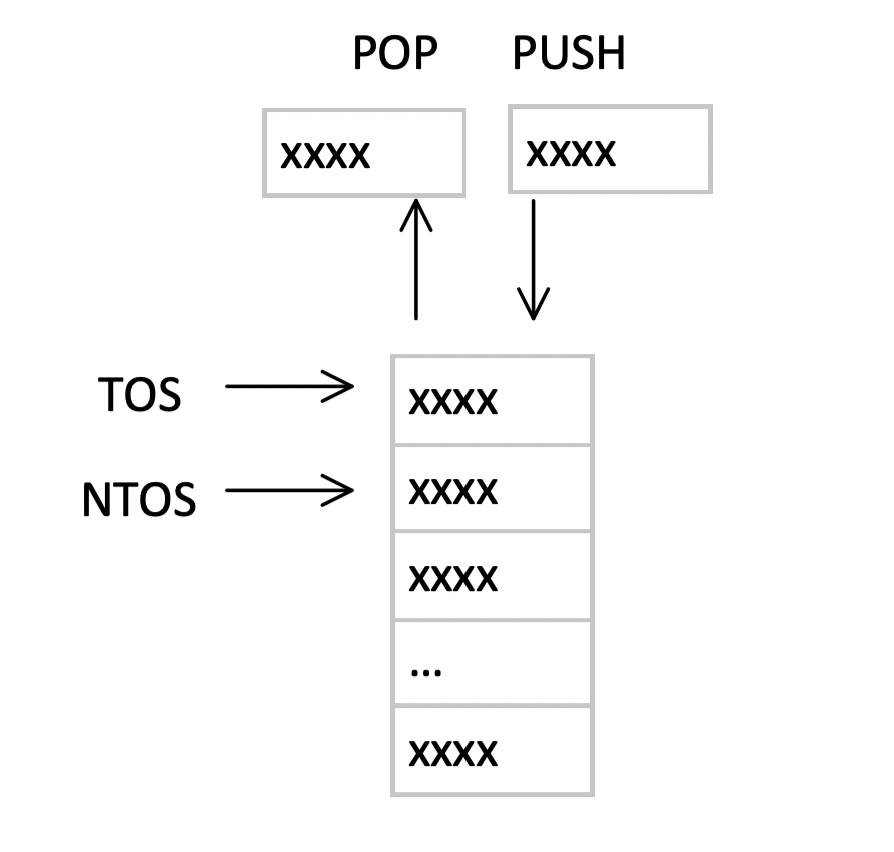
\includegraphics[scale=0.6]{Toxic_Stack_Model.png}
        \caption{Toxic Stack Model}
        \label{figure:stack_model}
    \end{figure}

    \subsection{Another Stack for Addressing Bus (Under Revising Now, Content Deprecated)}
    

    
    \subsection{Memory}
    The memory of the Toxic processor is accessed through Bus and only takes part of the addressing space. 
    The model of the Memory is different from common RAMs since for common RAMs, the block bit width is 1 bype (8 bits)
    while for the Toxic processor, the width of a block is half-byte (4 bits). \par
    For the Toxic processor, we assign the width of each block of the memory to be 4 bits.
    This memory model can be easily implemented using a standard memory block and would be discussed in detail in 
    Chapter \ref{chapter:implementation}.
    Detailed addressing space definitions can be found in detail in section \ref{section:addressingspace}.
    \subsection{Carry Bit}
    Carry Bit is a single bit register storing the carry of operations. There are three instructions that may possibly 
    generate a carry: ADD, LS, RS. Please refer to subsection \ref{subsection:add} for ADD, \ref{subsection:ls} for LS, 
    \ref{subsection:rs} for RS. In addition, the instruction CMP allows programmers to access the carry bit. Please Refer to
    \ref{subsection:cmp} for details.

    \section{Addressing Modes}
    There are three addressing modes in the Toxic processor:
    \begin{itemize}
        \item TOS (Top of Stack)
        \item NTOS (Next Top of Stack)
        \item Bus for memory and peripherals
    \end{itemize}

    \section{Addressing Space}
    These definitions for the addressing space is for the standard version of the Toxic processor.
    More versions of definitions of implementations can be found in Chapter \ref{chapter:implementation}
    \label{section:addressingspace}
    \subsection{Reserved: 0x0-0xf}
    \subsection{Code Memory: 0x10-0x7fff}
    \subsection{Data Memory: 0x8000-0xefff}
    \subsection{Peripherals: 0xf000-0xffff}

    \chapter{Instruction Set Architecture}
    \section{Instructions Map}
    \begin{table}[h]
        \begin{tabular}{|l|l|l|l|l|}
        \hline
        1:0\textbackslash{}3:2 & 00  & 01  & 11   & 10 \\ \hline
        00                     & P1  & POP & ADD  & SV \\ \hline
        01                     & P11  & DIS & NAND & LD \\ \hline
        11                     & CMP & SWP & LS   & B1 \\ \hline
        10                     & PC  & RVS & RS   & B0 \\ \hline
        \end{tabular}
    \end{table}
    For the explanation of instructions below, refer to Chapter \ref{chapter:design} for details
    about terminologies like Stack, Queue, pop, push, enqueue, dequeue, TOS, NTOS.
    \section{Push Instructions}
    \subsection{P1}
    \begin{itemize}
        \item Functionality: \textbf{Push} 0001 to stack.
        \item Expression:
        \begin{verbatim}
            Stack.push(0001);
        \end{verbatim}
    \end{itemize}

    \subsection{P11}
    \begin{itemize}
        \item Functionality: \textbf{Push} 0011 to stack.
        \item Expression:
        \begin{verbatim}
            Stack.push(0011);
        \end{verbatim}
    \end{itemize}

    \section{Stack and Bus Operation Instructions}
    \subsection{POP}
    \begin{itemize}
        \item Functionality: \textbf{Pop} from stack and
                \textbf{enqueue} the value \textbf{poped} from stack to the queue.
        \item Expression:
        \begin{verbatim}
            val = Stack.pop();
            Bus.push(val);
        \end{verbatim}
    \end{itemize}

    \subsection{DIS}
    \begin{itemize}
        \item Functionality: \textbf{Pop} from the stack and discard the value.
        \item Expression:
        \begin{verbatim}
            Stack.pop();
        \end{verbatim}
    \end{itemize}

    \subsection{SWP}
    \begin{itemize}
        \item Functionality: Swap the value of \textbf{TOS} and \textbf{NTOS}.
        \item Expression:
        \begin{verbatim}
            val = Stack.ntos;
            Stack.ntos = Stack.tos;
            Stack.tos = val;
        \end{verbatim}
    \end{itemize}

    \subsection{RVS}
    \begin{itemize}
        \item Functionality: \textbf{dequeue} from the Queue and \textbf{push} the value 
                    \textbf{dequeued} to the Stack.
        \item Expression:
        \begin{verbatim}
            val = Bus.pop();
            Stack.push(val);
        \end{verbatim}
    \end{itemize}

    \section{Numeric Computing Instructions}
    \subsection{ADD}
    \label{subsection:add}
    \begin{itemize}
        \item Functionality: \textbf{Push} the value of \textbf{TOS} + \textbf{NTOS}.
        \item Expression:
        \begin{verbatim}
            val = Stack.tos + Stack.ntos;
            Stack.push(val);
        \end{verbatim}
        \item Carry bit: 1 for addition having an carry, 0 for addition without an carry.
    \end{itemize}

    \subsection{NAND}
    \begin{itemize}
        \item Functionality: \textbf{Push} the value of \textbf{TOS} NAND (bit-wise) \textbf{NTOS}.
        \item Expression:
        \begin{verbatim}
            val = ~(Stack.tos & Stack.ntos);
            Stack.push(val);
        \end{verbatim}
    \end{itemize}

    \subsection{LS}
    \label{subsection:ls}
    \begin{itemize}
        \item Functionality: \textbf{Left Shift} one bit the value of \textbf{TOS}.
        \item Expression:
        \begin{verbatim}
            Stack.tos = Stack.tos << 1;
        \end{verbatim}
        \item Carry bit: carry bit equals the most significant bit of \textbf{TOS} \textbf{before shifting.} 
    \end{itemize}

    \subsection{RS}
    \label{subsection:rs}
    \begin{itemize}
        \item Functionality: \textbf{Right Shift} one bit the value of \textbf{TOS}.
        \item Expression:
        \begin{verbatim}
            Stack.tos = Stack.tos >> 1;
        \end{verbatim}
        \item Carry bit: carry bit equals the least significant bit of \textbf{TOS} \textbf{before shifting.} 
    \end{itemize}

    \section{Memory Operations Instructions}
    \subsection{SV}
    \begin{itemize}
        \item Functionality: \textbf{Save} the value of \textbf{TOS} to memory location 
                pointed by the \textbf{Bus} address.
        \item Expression:
        \begin{verbatim}
            Memory[BusAddress] = Stack.tos;
        \end{verbatim}
    \end{itemize}

    \subsection{LD}
    \begin{itemize}
        \item Functionality: \textbf{Push} the value of at memory location 
                pointed by the \textbf{Bus} address to the \textbf{Stack}.
        \item Expression:
        \begin{verbatim}
            Stack.push(Memory[BusAddress]);
        \end{verbatim}
    \end{itemize}

    \section{Branch Instructions}
    \subsection{B1}
    \begin{itemize}
        \item Functionality: Branch to the address pointed by the \textbf{Bus} 
                address if the least significant bit of \textbf{TOS} is 1.
        \item Expression:
        \begin{verbatim}
            if(Stack.tos[0] == 1)
            {
                PC = BusAddress;
            }
        \end{verbatim}
    \end{itemize}

    \subsection{B0}
    \begin{itemize}
        \item Functionality: Branch to the address pointed by the \textbf{Bus} 
                address if the least significant bit of \textbf{TOS} is 0.
        \item Expression:
        \begin{verbatim}
            if(Stack.tos[0] == 0)
            {
                PC = BusAddress;
            }
        \end{verbatim}
    \end{itemize}

    \section{Special Instructions}
    \subsection{CMP}
    \label{subsection:cmp}
    \begin{itemize}
        \item Functionality: Compare \textbf{TOS} and \textbf{NTOS} with the assumption 
                that they are both signed values, push an output (described below) to the Stack.
        \item Output[0] equals 1 for \textbf{TOS} == \textbf{NTOS}, equals 0 otherwise.
        \item Output[1] equals 1 for \textbf{TOS} > \textbf{NTOS}, equals 0 otherwise.
        \item Output[2] equals 1 for \textbf{TOS} < \textbf{NTOS}, equals 0 otherwise.
        \item Output[3] equals 1 for Numeric operation having an carry, equals 0 otherwise.
                        ADD, LS, RS are the three instructions that can possibly generate a carry.
                        Please refer to subsection \ref{subsection:add} for ADD, \ref{subsection:ls} for LS, 
                        \ref{subsection:rs} for RS.
        \item Expression:
        \begin{verbatim}
            output0 = Stack.tos == Stack.ntos;
            output1 = Stack.tos > Stack.ntos;
            output2 = Stack.tos < Stack.ntos;
            output3 = carry;
            Output = output0 + output1 << 1 
                    + output2 << 2 + output3 << 3;
            Stack.push(Output);
        \end{verbatim}
    \end{itemize}

    \subsection{PC}
    \begin{itemize}
        \item Important Note: This Instruction is optional for the most simplistic design.
        \item Functionality: Replace the whole \textbf{BusAddress} with current \textbf{PC} (Program Counter). 
                Please refer to Section \ref{section:pc} for more details about PC.
        \item Recall that \textbf{BusAddress} is part of the \textbf{Queue}. Please refer to \ref{subsection:queue}
                for more details about BusAddress and Queue.
        \item Expression:
        \begin{verbatim}
            BusAddress = PC;
        \end{verbatim}
    \end{itemize}


    \chapter{Micro-Architecture}
    \label{chapter:implementation}
    \section{Modules List}
    \begin{itemize}
        \item PC: Program Counter
        \item Instruction Memory
        \item Data Memory
        \item Queue
        \item Stack
        \item Controller
        \item ALU
    \end{itemize}
    \section{PC: Program Counter}
    \label{section:pc}
    \section{Instruction Memory}
    \section{Data Memory}
    \section{Queue}
    \section{Stack}
    \section{Controller}
    \section{ALU}
    \section{Diagram}

    \chapter{Assembly Language}
    In this chapter we will talk about how to write assembly code for the Toxic processor
    in a programmer's perspective. Useful Examples will also be provided.
    \section{Format}
    \begin{itemize}
        \item Each Instruction should take one line.
        \item Put comments after ";".
        \item Use "," to connect several instructions in one line.
        \item Use ":" to tag an location in code memory.
        \item All pseudo code start with "\$".
        \item The parameter of pseudo code is specified by "\#".
    \end{itemize}
    
    \section{Pseudo Codes}
    \subsection{\$PUSH}
    \begin{itemize}
        \item Usage: \$PUSH\#xxxx
        \item Functionality: Push "xxxx" to Stack
        \item Example: \$PUSH\#1010
    \end{itemize}
    \subsection{\$JMP}
    \begin{itemize}
        \item Usage: \$JMP\#[Flag or numeric offset]
        \item Functionality: Jump to the Flag or PC+offset
        \item Example1: \$JMP\#end
        \item Example2: \$JMP\#-5
    \end{itemize}
    \subsection{\$BEQ}
    \begin{itemize}
        \item Usage: \$BEQ\#[Flag or numeric offset]
        \item Functionality: Branch to the Flag or PC+offset if TOS equals NTOS.
        \item Example1: \$BEQ\#end
        \item Example2: \$BEQ\#-5
    \end{itemize}
    \subsection{\$BG}
    \begin{itemize}
        \item Usage: \$BG\#[Flag or numeric offset]
        \item Functionality: Branch to the Flag or PC+offset if TOS is greater than NTOS.
        \item Example1: \$BG\#end
        \item Example2: \$BG\#-5
    \end{itemize}
    \subsection{\$BL}
    \begin{itemize}
        \item Usage: \$BL\#[Flag or numeric offset]
        \item Functionality: Branch to the Flag or PC+offset if TOS is less than NTOS.
        \item Example1: \$BL\#end
        \item Example2: \$BL\#-5
    \end{itemize}
    \subsection{\$BC}
    \begin{itemize}
        \item Usage: \$BC\#[Flag or numeric offset]
        \item Functionality: Branch to the Flag or PC+offset if there is a carry.
        \item Example1: \$BC\#end
        \item Example2: \$BC\#-5
    \end{itemize}
    \subsection{\$ADDD}
    \begin{itemize}
        \item Usage: \$ADDD
        \item Functionality: Push $(TOS + NTOS)$ to Stack while discarding last TOS and NTOS.
        \item Example: \$ADDD
    \end{itemize}
    \subsection{\$ORD}
    \begin{itemize}
        \item Usage: \$ORD
        \item Functionality: Push $(TOS | NTOS)$ to Stack while discarding last TOS and NTOS.
        \item Example: \$ORD
    \end{itemize}
    \subsection{\$ANDD}
    \begin{itemize}
        \item Usage: \$ANDD
        \item Functionality: Push $(TOS \& NTOS)$ to Stack while discarding last TOS and NTOS.
        \item Example: \$ANDD
    \end{itemize}
    \subsection{\$NANDD}
    \begin{itemize}
        \item Usage: \$NANDD
        \item Functionality: Push $\overline{(TOS \& NTOS)}$ to Stack while discarding last TOS and NTOS.
        \item Example: \$NANDD
    \end{itemize}
    \subsection{\$DUP}
    \begin{itemize}
        \item Usage: \$DUP
        \item Functionality: Push the value of current TOS to Stack. (Duplicate TOS)
        \item Example: \$DUP
    \end{itemize}

    \section{Useful Examples: Without Pseudo Code}
    \subsection{Push 0000 to Stack}
    Number of Instructions: 2
    \begin{verbatim}
        P1 ; TOS now is 0001
        RS ; 0001 >> 1 = 0000
    \end{verbatim}

    \subsection{Push 1110 to Stack}
    Number of Instructions: 10
    \begin{verbatim}
        P11; TOS now is 0011
        LS,LS; TOS now is 1100
        P1,LS; TOS now is 0010, NTOS now is 1100
        ADD; Stack is: 1110, 0010, 0011
        SWP,DIS,SWP,DIS; discard 0010 and 0011
        ;now TOS is 1110
    \end{verbatim}

    \subsection{Push current TOS to Stack (Duplicate TOS)}
    Number of Instructions: 5
    \begin{verbatim}
        P1, RS; Push 0000 to Stack
        ADD; TOS + 0000 = TOS
        SWP, DIS; discard 0000
    \end{verbatim}

    \subsection{Perform AND operation (Bitwise)}
    Number of Instructions: 9
    $$X or Y = (XnandY)nand(XnandY)$$
    \begin{verbatim}
        ; Suppose TOS is 1010 and NTOS is 1100
        NAND ; TOS = ~(1010 & 1100) = 0111
        P1, RS, ADD, SWP, DIS; duplicate TOS 
        NAND ; TOS = ~(0111 & 0111) = 1000
        SWP, DIS; discard 0111 we duplicated
    \end{verbatim}

    \subsection{Perform OR operation (Bitwise)}
    Number of Instructions: 25
    $$XorY = (XnandX)nand(YnandY)$$
    \begin{verbatim}
        ; Suppose TOS is 1010 and NTOS is 1100
        P1, RS, ADD, SWP, DIS; duplicate TOS 
        NAND; TOS = 1010 nand 1010 = 0101
        POP; reserve the current TOS in Queue
        DIS, SWP; discard duplicated 1010
        ;then put 1100 on Top
        P1, RS, ADD, SWP, DIS; duplicate 1100
        NAND; TOS = 1100 nand 1100 =  0011
        POP; reserve the current TOS in Queue
        DIS, SWP; make the original Stack Intact
        RVS, RVS; restore 0101 and 0011 from Queue
        NAND; perform nand operation
        ; now, TOS = 1010 or 1100 = 1110
        SWP, DIS, SWP, DIS; discard 0101 and 0011
    \end{verbatim}

    \section{Useful Examples: With Pseudo Code}

\end{document}
